\documentclass{scrartcl}

\usepackage[utf8]{inputenc}
\usepackage{ngerman}
\usepackage{amsmath}
\usepackage{amssymb}
\usepackage{a4wide}
\usepackage{todonotes}
\usepackage{graphicx}
\usepackage{tikz}
\usepackage{pgfplots}

\def\layersep{2.5cm}

\begin{document}

\section{Perceptrons}

\begin{itemize}
  \item Modell eines künstlichen Neurons
  \item Vorgänger der \emph{Sigmoid Neurons}, die in heutigen modernen neuronalen Netzen benutzt werden
\end{itemize}

\begin{center}
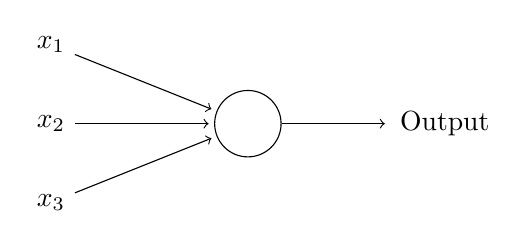
\begin{tikzpicture}[->, shorten >= 2pt]
  \tikzstyle{neuron}=[circle,draw,minimum size=24pt, inner sep=0pt]

  \foreach \name / \y in {1,...,3}
    \node (I-\name) at (0,-\y) {$x_{\name}$};

  \foreach \name / \y in {1,...,1}
    \node[neuron] (H1-\name) at (\layersep,-\y-1) {};

  \node (O) at (2*\layersep, -2) {Output};

  \foreach \source in {1,...,3}
    \foreach \dest in {1,...,1}
      \path (I-\source) edge (H1-\dest);

  \foreach \source in {1,...,1}
    \path (H1-\source) edge (O);
\end{tikzpicture}
\end{center}

\begin{itemize}
  \item \underline{Eingaben:} $x_1, x_2, \ldots, x_n \in \lbrace 0, 1 \rbrace$
  \item \underline{\emph{Weights}:} $w_1, w_2, \ldots, w_n \in \mathbb{R}$ für jede Eingabe $x_1$, der die jeweilige Eingabe gewichtet
  \item $\text{Output} = \begin{cases}
      0, & \text{wenn }\sum_j w_jx_j \leq \text{Treshold, wobei Treshold} \in \mathbb{R}\\
    1, & \text{sonst}
  \end{cases}$
  \item \textbf{vereinfachte Schreibweise:}
  \begin{itemize}
    \item $\sum_j w_j x_j = w \cdot x$, wobei $w$ und $x$ nun Vektoren beschreiben, dessen Komponenten die Gewichte und Eingaben sind
    \item ziehe den Treshold auf die andere Seite der Ungleichung (\emph{Bias}: $b = - \text{Treshold}$)
    \item $\Rightarrow$ Bias beschreibt, wie einfach es ist ein Perceptron auf $1$ zu bringen
    \item $\text{Output} = \begin{cases}
      0, & \text{wenn }w \cdot x + b \leq 0\\
      1, & \text{sonst}
    \end{cases}$
  \end{itemize}
\end{itemize}

\begin{itemize}
  \item Mit Hilfe eines \emph{neuronalen Netzes} aus Perceptons können kompliziertere Entscheidungen getroffen werden:
\end{itemize}

\begin{center}
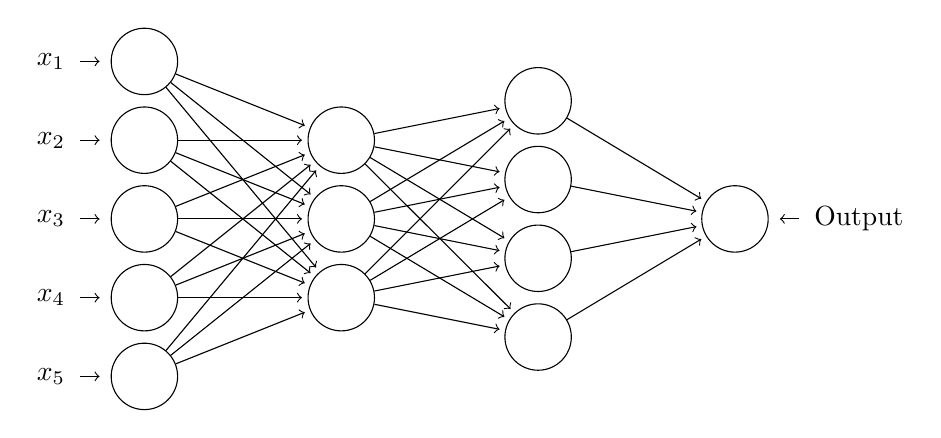
\begin{tikzpicture}[->, shorten >= 2pt]
  \tikzstyle{every pin edge}=[<-,shorten <= 4pt]
  \tikzstyle{neuron}=[circle,draw,minimum size=24pt, inner sep=0pt]

  \foreach \name / \y in {1,...,5}
    \node[neuron,pin=left:$x_{\y}$] (I-\name) at (0,-\y) {};

  \foreach \name / \y in {1,...,3}
    \node[neuron] (H1-\name) at (\layersep,-\y-1) {};

  \foreach \name / \y in {1,...,4}
    \path[yshift=-0.5cm]
      node[neuron] (H2-\name) at (2*\layersep,-\y) {};

  \node[neuron,pin=right:Output] (O) at (3*\layersep, -3) {};

  \foreach \source in {1,...,5}
    \foreach \dest in {1,...,3}
      \path (I-\source) edge (H1-\dest);

  \foreach \source in {1,...,3}
    \foreach \dest in {1,...,4}
      \path (H1-\source) edge (H2-\dest);

  \foreach \source in {1,...,4}
    \path (H2-\source) edge (O);
\end{tikzpicture}
\end{center}

\begin{itemize}
  \item neuronales Netz besteht aus drei Schichten: \emph{Input-Layer}, \emph{Hidden-Layer} und \emph{Output-Layer}
  \item \underline{Ziel:} bringe das Netz dazu zu lernen, d.h.\ ihre Weights und Bias-Werte anzupassen, sodass für jede Eingabe das erwartete Ergebnis erzielt wird
\end{itemize}

\section{Sigmoid Neurons}

\begin{itemize}
  \item \underline{Anforderung:} Eine kleine Änderung in den Weights/Bias-Werten führt nur zu einer kleinen Änderung in der Ausgabe
  \item $\Rightarrow$ Perceptrons sind dafür nicht geeignet, da sie nur flippen können
  \item \emph{Sigmoid Neurons}:
  \begin{itemize}
    \item \underline{Eingaben:} $x_1, x_2, \ldots, x_n \in [0, 1]$
    \item \underline{Ausgabe:} $\sigma(w \cdot x + b) = \sigma(z) = \frac{1}{1+e^{-z}}$
    \item \underline{Ähnlichkeit:} $z \rightarrow \infty \Rightarrow \sigma(z) \approx 1$ und $z \rightarrow - \infty \Rightarrow \sigma(z) \approx 0$
  \end{itemize}
\end{itemize}

\begin{center}
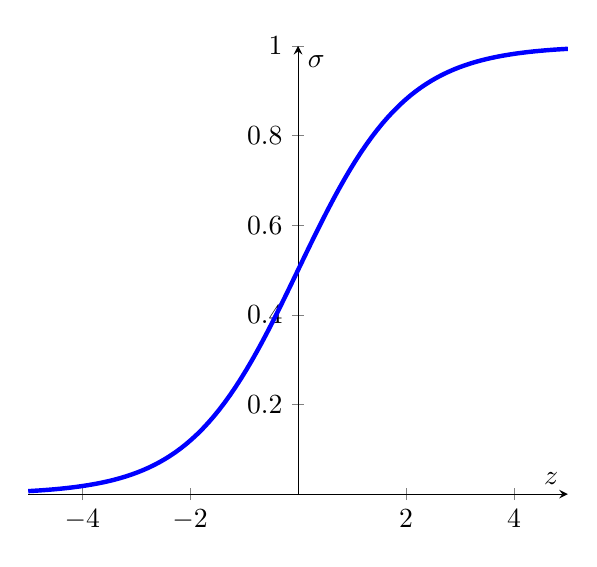
\begin{tikzpicture}
  \begin{axis}[
      axis lines=middle,
      xmax=5,
      xmin=-5,
      ymin=0,
      ymax=1,
      xlabel={$z$},
      ylabel={$\sigma$},
    ]
    \addplot [samples=100, ultra thick, blue] {1/(1+exp(-x))};
  \end{axis}
\end{tikzpicture}
\end{center}

\section{Neuronale Netze}

\begin{itemize}
  \item \textbf{Beispiel:} Schrifterkennung
  \begin{itemize}
    \item \underline{Eingabe:} 28 Pixel $\times$ 28 Pixel = 784 Eingaben mit Intensität $\in [0,1]$
    \item \underline{Ausgabe:} 10 Ausgabeneuronen, die die Wahrscheinlichkeiten beschreiben, dass das Bild die entsprechende Zahl zeigt, d.h.\ $\text{Output} > 0.5$
    \item \underline{Ziel:} approximiere die Funktion $y(x)$, die die Trainingdaten beschreibt, d.h.\ $y(x) = {(1, 0, 0, 0, 0, 0, 0, 0, 0, 0)}^T$ für ein Bild $x$ mit einer Null, usw.
    \item \underline{Methode:} minimiere Kostenfunktion $C(w,b) = \frac{1}{n} \sum_x || y(x) - a(x) ||^2$, wobei $a(x)$ der Output des neuronalen Netzes bei Input $x$ ist
  \end{itemize}
\end{itemize}

\end{document}
